% !TEX root =  ../main_manuscript.tex

\section{Demonstration of Personalized Schedules}
\label{sec : pers_schedule_PRIAS}
To demonstrate the personalized schedules, we apply them to the patients enrolled in PRIAS study. To this end, we divide the PRIAS dataset into a training part (5264 patients) and a demonstration part (three patients). We fit a joint model to the training dataset and then use it to create schedules for the demonstration patients. We fit the joint model using the R package \textbf{JMbayes} \citep{rizopoulosJMbayes}, which uses the Bayesian approach for parameter estimation.

\subsection{Fitting the Joint Model to the PRIAS Dataset}
\label{subsec : jm_fit_prias}
For each of the PRIAS patients, we know their age at the time of inclusion in AS, PSA history and the time interval in which GR is detected. For the longitudinal analysis of PSA we use $\log_2 \mbox{PSA}$ measurements instead of the raw data \citep{nieboer2015nonlinear}. The longitudinal sub-model of the joint model we fit is given by:
\begin{equation}
\label{eq : long_model_prias}
\begin{aligned}
\log_2 \mbox{PSA}_i(t) &= \beta_0 + \beta_1 (\mbox{Age}_i-70) + \beta_2 (\mbox{Age}_i-70)^2 + \sum_{k=1}^4 \beta_{k+2} B_k(t,\mathcal{K})\\ 
&+  b_{i0} + b_{i1} B_7(t, 0.1) + b_{i2} B_8(t, 0.1) +
\varepsilon_i(t),
\end{aligned}
\end{equation}
where $B_k(t, \mathcal{K})$ denotes the $k$-th basis function of a B-spline with three internal knots at $\mathcal{K} =\{0.1, 0.5, 4\}$ years, and boundary knots at zero and seven (0.99 quantile of the observed follow-up times) years. The spline for the random effects consists of one internal knot at 0.1 years and boundary knots at zero and seven years. For the relative risk sub-model the hazard function we fit is given by:
\begin{equation}
\label{eq : hazard_prias}
h_i(t) = h_0(t) \exp\big\{\gamma_1 (\mbox{Age}_i-70)  + \gamma_2 (\mbox{Age}_i-70)^2 + \alpha_1 m_i(t) + \alpha_2 m'_i(t)\big\},
\end{equation}
where $\alpha_1$ and $\alpha_2$ are measures of strength of the association between hazard of GR and $\log_2 \mbox{PSA}$ value $m_i(t)$ and $\log_2 \mbox{PSA}$ velocity $m'_i(t)$, respectively.

From the fitted joint model we found that $\log_2 \mbox{PSA}$ velocity and the age at the time of inclusion in AS were significantly associated with the hazard of GR. For any patient, an increase in $\log_2 \mbox{PSA}$ velocity from -0.10 to 0.14 (first and third quartiles of the fitted velocities, respectively) corresponds to a 2.02 fold increase in the hazard of GR. In terms of the predictive performance, we found that the area under the receiver operating characteristic curves \citep{landmarking2017} was 0.61, 0.65 and 0.59 at year one, year two, and year three of follow-up, respectively. Parameter estimates are presented in detail in Web Appendix C.

In PRIAS, the interval $l_i < T_i^* \leq r_i$ in which GR is detected depends on the PSA-DT of the patient. However, because the parameters are estimated using a full likelihood approach \citep{tsiatis2004joint}, the joint model gives valid estimates for all of the parameters, under the condition that the model is correctly specified (see Web Appendix A.2 and C.3). To this end, we performed several sensitivity analysis in our model (e.g., changing the position of the knots, etc.) to investigate the fit of the model and also the robustness of the results. In all of our attempts, the same conclusions were reached, namely that the $\log_2 \mbox{PSA}$ velocity is more strongly associated with the hazard of GR compared to the $\log_2 \mbox{PSA}$ levels.

\subsection{Personalized Schedules for the First Demonstration Patient}
\label{subsec : demo_prias_pers_schedule}
We now demonstrate the functioning of the personalized schedules for the first demonstration patient (see Web Appendix D for the other two demonstration patients). The fitted and observed $\log_2 \mbox{PSA}$ profile, time of latest biopsy and proposed biopsy times $u$ for him are shown in the top panel of Figure \ref{fig : prias_demo_pid_911}. We can see that with a consistently decreasing PSA and negative repeat biopsy between year three and year 4.5, the proposed time of biopsy based on the dynamic risk of GR has increased from 3.05 years ($\kappa=0.94$) to 13.73 years ($\kappa=0.96$) in this period. The proposed time of biopsy based on expected time of GR has also increased from 14.22 years to 16.07 years. We can also see in the bottom panel of Figure \ref{fig : prias_demo_pid_911} that after each negative repeat biopsy, $\mbox{SD}[T^*_j] = \sqrt{\mbox{var}_g(T^*_j)}$ decreases sharply. Thus, if the expected time of GR based approach is used, then the offset $O^S_j$ will be smaller on average for biopsies scheduled after the second repeat biopsy than those scheduled after the first repeat biopsy.

\begin{figure}
\centerline{
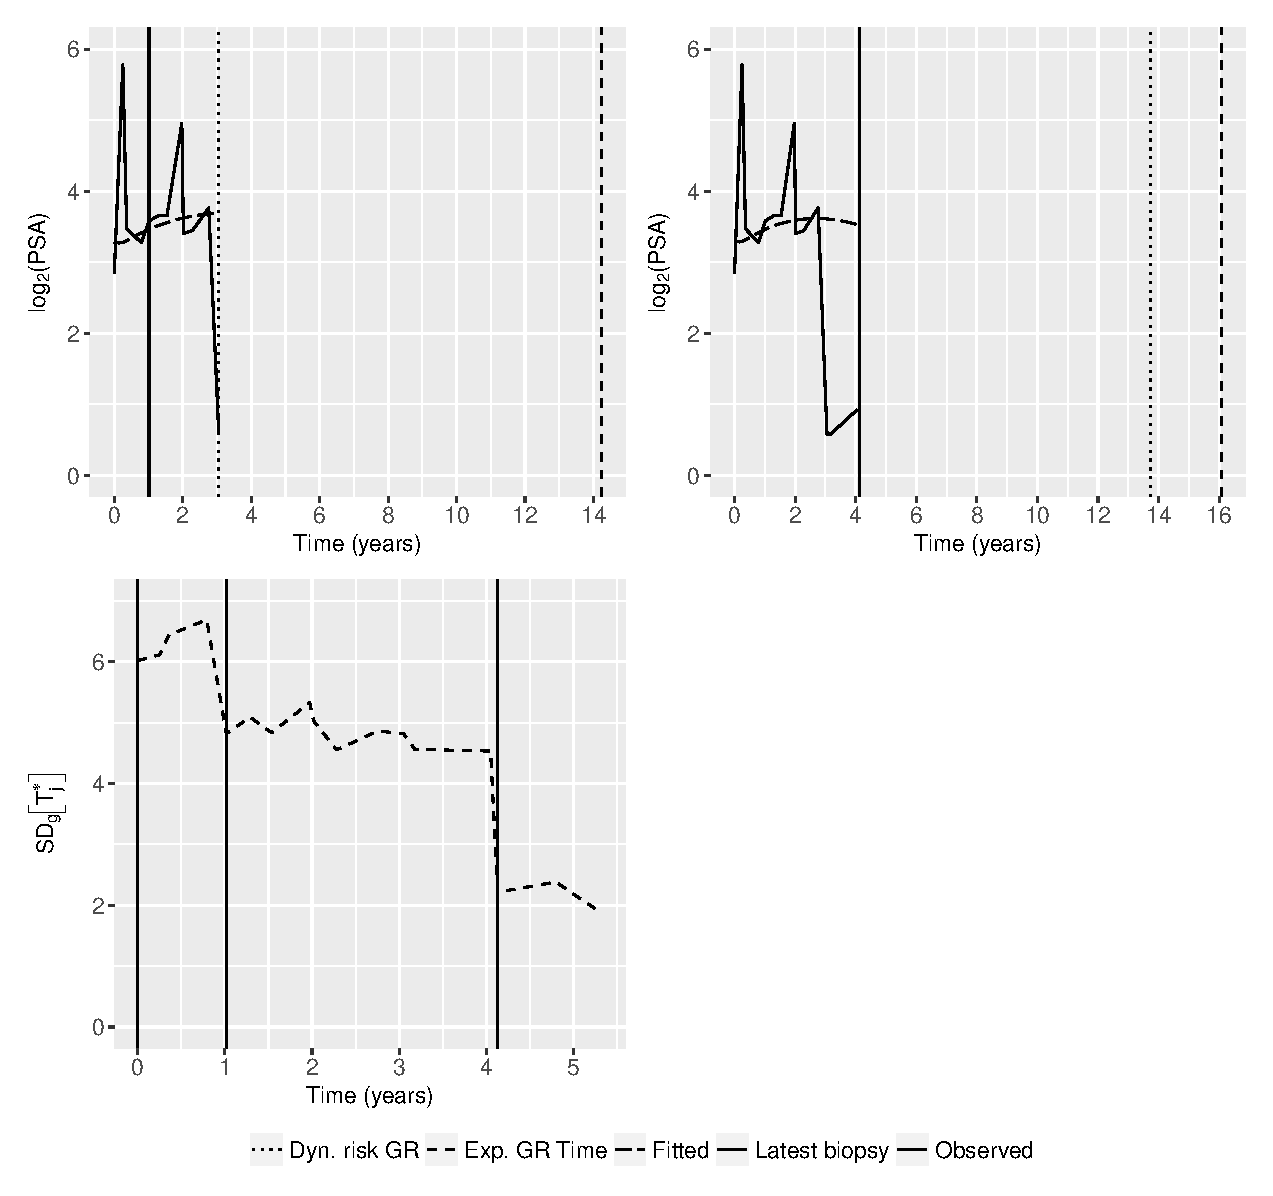
\includegraphics[width=\columnwidth]{images/prias_demo/case_911_t3.eps}
}
\caption{Top panel: Fitted versus observed $\log_2 \mbox{PSA}$ profile, history of repeat biopsies and corresponding personalized schedules for the first demonstration patient. Bottom Panel: History of repeat biopsies and standard deviation $\mbox{SD}_g(T^*_j) = \sqrt{\mbox{var}_g(T^*_j)}$ of the posterior predictive distribution of time of GR over time for the first demonstration patient.}
\label{fig : prias_demo_pid_911}
\end{figure}